% ============================================================================
%  Thesis B — First complete LaTeX draft
%  Working title: Measurement Discipline for ML Diagnostics:
%                 A Psychometric Framework with a LoRA-Merging Case Study
%
%  Status: first complete prose pass. Follows the section structure and
%  length budget of draft_v2_thesis_b_outline.md. Expected to go through
%  at least one revision cycle before venue submission; see
%  revision_notes.md RN-012 for the repositioning record and the outline
%  for per-section intent.
%
%  Compile:
%    pdflatex draft_v2_thesis_b
%    bibtex   draft_v2_thesis_b
%    pdflatex draft_v2_thesis_b
%    pdflatex draft_v2_thesis_b
%
%  This draft uses a generic article class with 1-inch margins; the
%  venue-specific template swap happens when the venue is locked.
% ============================================================================

\documentclass[11pt]{article}

\usepackage[letterpaper,margin=1in]{geometry}
\usepackage[T1]{fontenc}
\usepackage[utf8]{inputenc}
\usepackage{amsmath,amssymb}
\usepackage{graphicx}
\usepackage{booktabs}
\usepackage{caption}
\usepackage{natbib}
\usepackage{microtype}
\usepackage{hyperref}
\hypersetup{colorlinks=true, linkcolor=black, citecolor=black, urlcolor=black}

\bibliographystyle{plainnat}

\title{Measurement Discipline for ML Diagnostics:\\
  A Psychometric Framework with a LoRA-Merging Case Study}
\author{Anonymized\thanks{De-anonymized references in the tagged
    repository; see \texttt{n134-submission-draft-v1}.}}
\date{April 2026}

\begin{document}
\maketitle

\begin{abstract}
ML diagnostic metrics --- scores claimed to predict model behavior,
merging outcomes, training dynamics, or capability --- are routinely
reported as point estimates to three or four decimal places without
the measurement-theoretic infrastructure that psychological assessment
has treated as baseline methodology for decades. We argue that this
practice systematically overclaims precision and generality, and we
introduce a framework for applying classical measurement theory
(reliability coefficients, standard error of measurement, confound
decomposition, pre-registered decision rules with explicit tolerance
schedules) to ML diagnostic reporting. We demonstrate the framework
through a pre-registered decoder-scale study of spectral LoRA-merging
diagnostics ($N = 45$ cross-task adapter pairs on Mistral-7B-v0.3),
which produces a null on per-pair merge prediction under
family-confound control, replicates task-boundary detection across
three architectures and two metric families, and --- in the course of
being subjected to measurement-discipline scrutiny --- surfaces a
previously unnamed property of the primary test statistic: rank-based
correlations on small-$N$ residuals have intrinsic floating-point
precision of order $10^{-2}$, comparable to their sampling variability.
We argue this last observation is not an incidental finding but an
instance of the paper's central claim: measurement discipline applied
to ML diagnostics produces findings that unstructured reporting would
not surface.
\end{abstract}

\section{Introduction}
\label{sec:introduction}

\subsection{The reporting gap}

A recurring pattern in the ML methods literature is to report a
diagnostic metric as a point estimate to three or four decimal
places without any accompanying description of its measurement
properties --- without a reliability coefficient that would say how
stable the score is across seeds or calibration data, without an
explicit tolerance schedule that would say how much of the reported
precision is substantive, and without a pre-registered confound
decomposition that would distinguish the diagnostic's explanatory
share from that of simpler alternatives. Two examples illustrate
the pattern; the convergence between them across subfields is the
feature we want to draw out.

Consider a representative claim from the LoRA-merging literature.
\citet{zhou2026demystifying} report that, across 190 task pairs on
ViT-B/32 classifiers, an activation-based pairwise diagnostic
predicts merge outcome with $r = 0.572$ (TSV, the strongest
individual method among those evaluated). The value is stated to
three significant figures. No cross-seed reliability coefficient
accompanies it: the stability of the correlation when the
activation-calibration set is resampled, or when adapters trained
under different seeds are substituted, is not reported. No tolerance
schedule states how much of the third digit is substantive and how
much is sampling variability or implementation sensitivity. No
pre-registered confound decomposition distinguishes the diagnostic's
explanatory share from what task-family identity alone might
capture; the correlation is presented as if the diagnostic were its
sole relevant explanans. The point is not that $0.572$ is wrong ---
it may well be the best available estimate from the reported
experiment --- but that the reporting convention treats a
point-estimate correlation as a self-standing measurement rather
than as the central claim of an instrument whose reliability,
precision, and confound structure have been independently
characterized.

%
% TODO(§1.1 second example): the capability-evaluation characterization
% below is argumentatively defensible as a pattern-description, but
% a specific cited claim would strengthen it. Candidate directions:
% (a) a method-paper leaderboard claim reporting MMLU/BBH to two or
% three decimals; (b) the capability-evaluation reliability literature
% (e.g., Burnell et al. 2023 on reporting practice; Balloccu et al. on
% contamination); (c) a specific probing-accuracy or faithfulness
% claim from the interpretability literature. Any swap requires
% verifying the exact reported value and adding the bib entry.
%
The same pattern appears outside the merging literature. Capability-
evaluation scores on standard benchmarks --- MMLU, HellaSwag,
BIG-Bench-Hard, and their successors --- are routinely reported to
two or three decimal places of accuracy without cross-seed or
cross-prompt reliability coefficients, without explicit tolerance
schedules for the reported digits, and without pre-registered
confound controls that would distinguish improvements attributable
to a claimed intervention from those attributable to prompt-format
sensitivity, evaluation-metric choice, or evaluation-set
contamination. That the same measurement-theoretic context is
missing in a subfield with no methodological contact with
LoRA-merging research suggests the gap is not an idiosyncrasy of
one community but a general feature of how ML diagnostics are
currently reported.

Three specific gaps follow from this pattern. Reliability
coefficients in the classical-test-theory sense --- ICC, SEM,
coefficient alpha or its distribution-based analogues --- are
nearly absent from ML diagnostic reports. Point estimates are
quoted to three or four decimals without uncertainty bounds
calibrated to the actual dependence structure of the data. Confound
decomposition is rare, and when present is usually conducted
post-hoc rather than pre-registered. Each of these gaps on its own
is repairable by a careful reviewer; collectively, they produce a
literature in which a reader who wants to know how much credence to
place in a reported value has no reliable way to calibrate.

\subsection{The psychometric analog}

Psychological assessment has confronted the same class of problem
since at least the 1950s, and has developed a coordinated set of
methods to address it. An instrument's reliability is treated as a
first-class property, measured empirically and reported alongside any
substantive claim \citep{cronbach1951alpha,shrout1979icc}. Standard
error of measurement --- the expected deviation of a single
observation from its true score under the instrument's reliability
--- is the decimal-place precision claim, calibrated to the
instrument rather than quoted by convention. Construct validity ---
the discipline of defending that an instrument measures what its
name claims it measures, distinct from operationalization ---
operates as a unified theory of scoring inference rather than as an
ad-hoc checklist \citep{messick1995validity,cronbachmeehl1955}.
None of these concepts is novel, and none is specific to psychology;
what is specific to psychology is the systematic expectation that
every reported diagnostic value carries this measurement-theoretic
context.

ML has drawn on this tradition less than it could. The framework we
propose in Section~\ref{sec:framework} is not a claim of conceptual
originality but a proposal for systematic, coordinated application
of measurement-theoretic methods to ML diagnostic reporting.

\subsection{Contribution claims}

\begin{enumerate}
  \item A four-component framework for applying measurement discipline
    to ML diagnostics: (i) construct validity, (ii) reliability
    coefficients, (iii) bounded precision claims with explicit
    tolerance schedules, and (iv) confound decomposition with
    pre-registered decision rules.
  \item A detailed worked example applying the framework to spectral
    LoRA-merging diagnostics: a pre-registered decoder-scale null on
    per-pair merge prediction under family-confound control, a
    three-architecture replication of task-boundary detection across
    two metric families, and a pre-registered four-method comparison.
  \item A specific previously-unnamed measurement property of partial
    Spearman correlations on small-$N$ residuals, surfaced by the
    measurement-discipline scrutiny the framework prescribes, with
    implications for any rank-based diagnostic metric reported at
    small sample sizes.
\end{enumerate}

\subsection{Road map}

Section~\ref{sec:framework} develops the framework.
Section~\ref{sec:case-study} introduces the worked example's setting.
Sections~\ref{sec:applying}--\ref{sec:rank-observation} present the
worked example. Section~\ref{sec:generalizing} returns to the
framework and generalizes from the case study to broader reporting
practice. Section~\ref{sec:objections} addresses limitations and
common objections to the thesis. Section~\ref{sec:conclusion}
concludes.

\section{A Measurement-Discipline Framework for ML Diagnostics}
\label{sec:framework}

Two views of what an ML diagnostic metric is stand behind the
reporting practices this paper addresses. On the first, which
operates implicitly in much of the ML methods literature, a score is
a direct readout of a latent property: the computation from model
weights, activations, or outputs reports what its name claims it
reports, and the only remaining measurement question is whether
noise has been adequately reduced. On the second, which the
psychometric tradition has developed since at least
\citet{cronbachmeehl1955}, a score is a fallible indicator: an
observable whose relationship to the theoretical object it is taken
to measure must be structurally defended rather than presumed. The
framework we propose in this section is what follows from replacing
the first view with the second.

The replacement is not a methods upgrade. It is a conceptual
reorientation whose consequences include a specific set of reporting
practices, but the practices are consequences rather than the
starting point. Treating a diagnostic as a fallible indicator
commits the author to defending, jointly and inseparably, four
things: what the score indicates, how stable the indication is, what
precision the indication can actually support, and what else could
explain the signal. These are not four independent methodological
virtues from among which an author may pick and choose; they are
four aspects of a single commitment, continuous with the unified
theory of construct validity
\citep{messick1989validity,messick1995validity} that psychometrics
has developed in the decades since \citet{cronbachmeehl1955}. An
author who omits any one tacitly reverts to the direct-readout view
at the point of omission, since a score whose stability, precision,
or alternative explanations go undefended is a score being treated
as though those defenses were unnecessary. The framework's internal
coherence is the argument; its component practices, taken
separately, are the ordinary stock of classical test theory and,
individually, could be adopted without challenging the default view
of what an ML diagnostic is.

We develop the four defenses in the order a reader's credence should
consult them. A reader asks of any score, first what it purports to
measure (§\ref{sec:framework-construct}), then how stable its
readings are (§\ref{sec:framework-reliability}), then what precision
those readings can support (§\ref{sec:framework-precision}), and
finally what else might be producing them
(§\ref{sec:framework-confound}). The ordering is epistemic rather
than logical --- the four defenses are jointly required, and no one
of them is prior to the others in the inferential argument --- but
it tracks the questions a careful reader's credence would need
resolved before taking a score as evidence for a substantive claim.

\subsection{What the score indicates}
\label{sec:framework-construct}

A diagnostic's \emph{theoretical object} is what the score is taken
to measure: a geometric property of two adapters' updates, a
capability's presence or absence, a training regime's character. Its
\emph{operationalization} is the specific computation that
instantiates the object. Under the inferential view the paper must
state both explicitly and defend the connection between them as a
separate argumentative step; under the direct-readout view the
distinction does not arise, because the operationalization is
treated as transparently identical to the object. The typical ML
failure mode is the conflation: a paper that says ``our spectral
alignment score predicts merge outcomes'' is usually reporting
results about the operationalization (a specific computation from
weights) as though they were results about the theoretical object
(the geometric relationship between two adapters' learned updates).
Under the inferential view the conflation is an error; under the
direct-readout view it is not even legible as one.

The distinction has empirical consequences. Different
operationalizations of the same theoretical object can produce
different predictive patterns on the same data. N07/N132's
subspace-principal-angle-based overlap metric and N133/N134's
singular-value-weighted cosine alignment both claim to measure
spectral similarity between two adapters' weight-space updates, but
their raw values lie on non-comparable scales, and cross-study
comparisons of the raw values are unsound without metric-family
harmonization. The psychometric tradition treats such harmonization
as part of construct validity in the unified-theory sense
\citep{messick1989validity}: the validity argument \emph{is} the
defense of the connection between theoretical object and chosen
operationalization, and no cross-operationalization claim is
licensed without it. Pre-registered articulation of the distinction
--- stating the theoretical object, the operationalization, and the
defense of their connection as three separate things --- is the
discipline that forces the harmonization to be explicit rather than
presumed.

\subsection{How stable the indication is}
\label{sec:framework-reliability}

A score has evidential weight only to the extent that it would
reproduce under replication of the conditions that produced it. For
an ML diagnostic computed from stochastic training processes, the
relevant replication is over training seeds, calibration-data
samples, and implementation details that vary across labs. An ML
diagnostic reported as ``$\rho = 0.573$'' without an accompanying
reliability coefficient is making an implicit claim that this second
question has been answered in the limit --- that the score is
perfectly reliable, in the sense that its reports do not vary across
replications --- which is almost never true and never licensed by
the report itself.

We make the recommendation specific rather than hortatory. For a
score computed per-adapter, cross-seed intraclass correlation
(ICC; \citealp{shrout1979icc}) is the natural coefficient, estimated
from three or more seeds per task; at two seeds the estimate has
confidence intervals whose width is itself informative about the
evidential weight of the score's reports. For a score computed
per-pair of models, the analog is cross-seed-pair ICC across pairs
that should be semantically equivalent (same task-pair, different
random seeds). The N134 design commits to three seeds per task
specifically to support this estimate. On this design the estimate
is $\hat{\rho}_{\mathrm{ICC}} = 0.566$ (moderate) with SEM $= 0.014$
and 95\% CI $[0.165, 0.874]$ by Shrout--Fleiss
(Appendix~\ref{app:reliability}), reported as the
instrument-validation step the framework requires.

\subsection{What precision the indication supports}
\label{sec:framework-precision}

A score reported as ``$-0.533$'' to three decimals makes an implicit
claim that its third decimal carries information. The claim may be
defensible from sampling variability alone; it is rarely defensible
once implementation sensitivity, cross-environment reproduction, and
intrinsic numerical properties of the statistic at the operative
sample size are considered. Bounded precision is the discipline of
stating what the uncertainty on the reported decimal is, calibrated
per source. The relevant calibration is not a single ``standard
error'' but a tolerance schedule: sampling variability,
implementation sensitivity, cross-environment reproduction, and
intrinsic-statistic precision each contribute, and which one
dominates depends on the statistic, the operative sample size, and
the reproduction condition.

Section~\ref{sec:rank-observation} develops the paper's most
striking instance: the worked example's headline statistic has
intrinsic floating-point precision of approximately $\pm 0.01$ at
$n = 45$, meaning its third decimal is not a real claim regardless
of what sampling variability the bootstrap confidence interval
reports. The observation is not about the bootstrap's calibration;
it is about the statistic's intrinsic precision on residuals at this
sample size. A single ``$\pm$'' would not have surfaced the
distinction. A tolerance schedule does.

\subsection{What else could explain the signal}
\label{sec:framework-confound}

The final defense is the discipline of distinguishing what a
diagnostic predicts from what is predictable by simpler alternatives
--- task identity, input length, surface features, known demographic
structure of the data, or in the present paper's worked example,
task-family-pair identity. Under the direct-readout view the
distinction is not load-bearing because the score's predictive
relationship to its object is presumed; under the inferential view
the distinction \emph{is} the test of the score's information over
and above alternatives. A score whose reported predictive
correlation is entirely accounted for by a simpler alternative has
not measured its purported object; it has measured the alternative.

Pre-registration of the decomposition is what distinguishes the
framework's confound-handling from the post-hoc version that
currently dominates. Post-hoc decomposition following a failed main
analysis reads as an excuse; pre-registered decomposition is a
commitment that the diagnostic must clear \emph{before} seeing the
data. The worked example in Section~\ref{sec:empirical} makes the
general form concrete with a family-pair residualization and a
$\Delta R^2$ threshold; we develop the specifics at the relevant
point of the worked example (Sections~\ref{sec:applying} and
\ref{sec:empirical-h1}) rather than in advance of it, to keep the
framework itself independent of the particulars of any single
application.

\section{Case Study: Spectral Diagnostics for LoRA Adapter Merging}
\label{sec:case-study}

Low-rank adaptation (LoRA) fine-tuning \citep{hu2021lora} has become
a standard method for task-adapting large pretrained models. A
practitioner who has accumulated multiple LoRA adapters for different
tasks often wishes to combine them into a single adapter that
supports all the original capabilities simultaneously. Adapter
merging --- typically a weighted linear combination of the adapter
weight deltas --- accomplishes this cheaply but can produce large
performance degradation on one or both source tasks.

A recent literature has proposed methods for improving merge
outcomes \citep{stoica2024knots,gargiulo2025tsv,li2026svc,
zhang2025osrm} and for predicting which adapter pairs are likely to
merge successfully \citep{zhou2026demystifying,rahamim2026mergeability,
bolton2026simmerge}. Decoder-scale empirical evaluations of these
methods have emerged in parallel \citep{hitit2026insystematic,
he2025mergebench}, typically reporting predictive correlations as
point estimates without the measurement-theoretic context
Section~\ref{sec:framework} requires.

Our worked example is a pre-registered decoder-scale study of one
such spectral diagnostic: O-module depth-weighted
singular-value-weighted alignment, denoted $S_{\mathrm{H1}}$. The
formal definition is in Appendix~\ref{app:score}. The LoRA-merging
setting is incidental to the paper's argument; the argument
would hold equally for interpretability scores, capability
evaluations, or any other ML diagnostic class. This section treats
the setting as background just sufficient for a reader outside the
merging subfield to follow the worked example.

\section{Applying the Framework: Pre-Registration and Design}
\label{sec:applying}

\subsection{Construct articulation for the spectral triage claim}

The theoretical object of $S_{\mathrm{H1}}$ is a geometric property
of two adapters' weight-space updates: specifically, the extent to
which their dominant singular directions occupy shared subspaces.
The operationalization is a specific computation from per-layer
singular value decompositions (Appendix~\ref{app:score}), weighted
by linear depth, restricted to the O-projection module. The choice
to focus on the O-projection and to use linear depth weighting
derives from precursor analyses (Gradience N133
\citep{anonymized2026n133}) which found that O-projection
same-cross separation was stronger than Q/K/V and that deeper layers
separated same-task from cross-task pairs more sharply than
shallower ones. Those observations do not establish that
$S_{\mathrm{H1}}$ is the best possible operationalization; they
license a choice among many plausible ones, and the pre-registration
commits to the specific choice before testing.

\subsection{Reliability considerations at pre-registration time}

The N134 design commits to three seeds per task across eight
pre-registered tasks, yielding 24 adapters. This design supports
cross-seed reliability estimation for $S_{\mathrm{H1}}$ as an
instrument: same-task adapter pairs (three same-task pairs per task,
24 total) provide the replicate structure that a cross-seed ICC
estimate requires. The resulting estimate,
$\hat{\rho}_{\mathrm{ICC}} = 0.566$ with SEM $= 0.014$, is
reported at Appendix~\ref{app:reliability}; for the purpose of the
pre-registered H1 test, the relevant observation is that the design
was calibrated to support this estimate before data collection began,
not that the estimate was examined post-hoc to reassure reviewers.

\subsection{Confound decomposition pre-registration}

Four confounds were identified during precursor analysis of N133 and
were pre-registered against in the N134 design
\citep{anonymized2026n134spec}:
\begin{itemize}
  \item \textbf{C1 source-metric dynamic range}: adapters trained to
    accuracy within a tight band (here, 0.70--0.90) to prevent
    source-accuracy residual from driving correlations.
  \item \textbf{C2 task-family partition}: eight tasks spanning five
    task families with no family exceeding two tasks; pre-registered
    family-pair labels used for residualization.
  \item \textbf{C3 within-task variance}: three seeds per task,
    enabling reliability estimation and distinguishing within-task
    variance from cross-task variance.
  \item \textbf{C4 post-hoc fitting}: the H1 score is pre-registered
    in the spec; no post-hoc search across alternative scores is
    permitted in the primary test.
\end{itemize}
The decision rule operationalizes C2 specifically: partial Spearman
$\rho$ between $S_{\mathrm{H1}}$ and the max-degradation outcome is
computed on OLS residuals after both variables are residualized on
the pre-registered family-pair labels (FAMILY\_B). The $\Delta R^2$
test quantifies the additional variance the geometric score explains
beyond family identity. The quantitative shares this decomposition
produces --- $88.1\%$ of outcome variance captured by family-pair
identity alone, $+0.003$ contributed by $S_{\mathrm{H1}}$ beyond it
(reported in full at Section~\ref{sec:empirical-h1}) --- are the
framework's confound-decomposition discipline made concrete, and are
what licenses the subsequent null as informative rather than
uninterpretable.

\subsection{Decision rule with explicit precision}

The pre-registered decision rule requires both: partial $\rho \geq
+0.50$ at $p < 0.05$, and $\Delta R^2 \geq 0.10$, with sign
constraint absolute (wrong sign fails regardless of magnitude).
Both thresholds are calibrated to practically meaningful effect sizes
for the triage decision the diagnostic is intended to support, not
to statistical-significance thresholds alone. A significant but
wrong-signed result is committed \emph{a priori} to be interpreted as
a null under the rule, not as a reversed confirmation.

\section{Worked Example: Empirical Results}
\label{sec:empirical}

The pre-registered H1 hypothesis on $S_{\mathrm{H1}}$ is not
confirmed. Three confirmatory replications of task-boundary detection
across architectures and metric families pass cleanly. A
pre-registered four-method comparison produces a regime null at the
evaluated sample size. Each subsection below subordinates the
empirical result to its framework-demonstration role.

\subsection{H1 outcome under the pre-registered rule}
\label{sec:empirical-h1}

Table~\ref{tab:h1-decision} reports the pre-registered decision
criteria and observed values. The partial correlation is large in
magnitude ($\rho = -0.533$, $p = 1.6 \times 10^{-4}$, bootstrap 95\%
CI under family-pair block resampling: $[-0.825, -0.131]$) but
opposite in sign to the pre-registered prediction. $\Delta R^2$
is $+0.003$, far below the 0.10 threshold.
Figure~\ref{fig:h1-decision} shows the underlying scatter with the
raw and family-residualized regression lines.

\begin{table}[h]
  \centering
  \small
  \begin{tabular}{lccc}
    \toprule
    Criterion & Required for H1 & Observed & Status \\
    \midrule
    Raw Spearman $\rho$ sign & positive & $-0.180$ & FAIL \\
    Partial $\rho$ (FAMILY\_B) & $\geq +0.50$, $p < 0.05$ & $-0.533$ ($p{=}1.6{\times}10^{-4}$) & FAIL (wrong sign) \\
    $\Delta R^2$ over FAMILY\_B baseline & $\geq 0.10$ & $+0.003$ & FAIL \\
    FAMILY\_B-only $R^2$ & --- & $0.881$ & (reference) \\
    \bottomrule
  \end{tabular}
  \caption{H1 decision criteria and observed values.}
  \label{tab:h1-decision}
\end{table}

\begin{figure}[h]
  \centering
  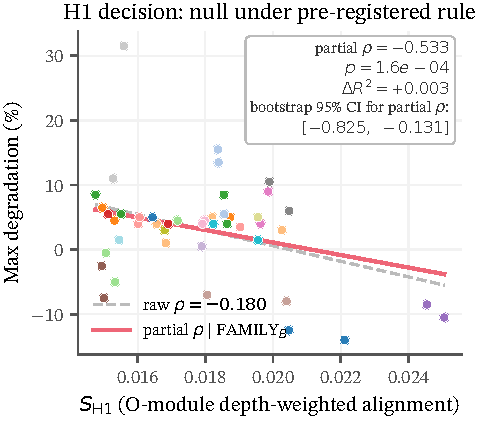
\includegraphics[width=0.7\textwidth]{figures/h1_decision.pdf}
  \caption{Scatter of $S_{\mathrm{H1}}$ against max post-merge
    degradation for the 45 evaluated cross-task pairs. Grey dashed
    line: raw OLS regression ($\rho = -0.180$). Red solid line:
    regression of max degradation on $S_{\mathrm{H1}}$ after both
    variables are OLS-residualized on FAMILY\_B dummies (partial
    $\rho = -0.533$). Point colors encode family-pair identity (28
    levels, \texttt{tab20} cycled) to make the family-level
    clustering visible; no individual-level legend is provided
    because 28 entries would be unreadable at this width. The partial
    correlation is large in magnitude but opposite in sign to the
    pre-registered prediction, and therefore fails the sign
    constraint of the decision rule regardless of magnitude.}
  \label{fig:h1-decision}
\end{figure}

Under the pre-registered rule, H1 is a null. The directional
information in the wrong-signed partial correlation is
hypothesis-generating but is excluded from licensing any conclusion
by the C4 pre-registration discipline; follow-up investigation of
four candidate interpretations (within-family over-commitment,
source-accuracy residual, inverted-substrate measurement,
intrinsic-mergeability) is out of scope for the present paper and
is the subject of a planned N135-alt study.

\subsection{Why this is an informative null, framework-wise}

Task-family-pair identity explains 88.1\% of outcome variance on
its own; $S_{\mathrm{H1}}$ contributes $+0.003$. Without the
framework's confound-decomposition discipline, the raw correlation
(also negative, smaller magnitude) would have been reported without
context, and the reader would have had no way to assess what
fraction of any predictive claim was actually family identity
operating under a different name. The informativeness of the null
is legible because the decomposition is pre-registered; it is
opaque otherwise. Readers interested in the informativeness
calculation should note that the $R^2 = 0.881$ figure is itself a
finding --- a large effect size for the simplest possible alternative
explanation --- and is reportable regardless of how the geometric
diagnostic performs.

\subsection{Three-architecture replication of task-boundary detection}

Three confirmatory replications of task-boundary detection pass
cleanly on N134 (Table~\ref{tab:replications}) and, combined with
prior results on DistilBERT \citep{anonymized2026n130} and DeBERTa
\citep{anonymized2026n132}, constitute a task-boundary detection
replication across three architectures and two metric families.

\begin{table}[h]
  \centering
  \small
  \begin{tabular}{llll}
    \toprule
    Claim & Observed & Threshold & Status \\
    \midrule
    B-P1 task-boundary overlap & 0/24 same below, 0/252 cross above midpoint & zero overlap & PASS \\
    B-P2 same/cross separation & ratio $2.28\times$; Welch $t=15.9$, $p=6{\times}10^{-14}$ & ratio $\geq 2.0$ & PASS \\
    B-P4 erank ANOVA across tasks & $F = 165.6$, $p = 1{\times}10^{-13}$ & $p \leq 10^{-6}$ & PASS \\
    \bottomrule
  \end{tabular}
  \caption{Confirmatory replications, all non-gating for H1 but
    reported per the pre-registration.}
  \label{tab:replications}
\end{table}

\begin{figure}[h]
  \centering
  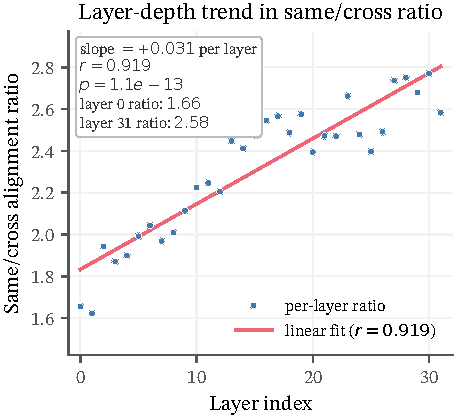
\includegraphics[width=0.6\textwidth]{figures/layer_depth_trend.pdf}
  \caption{Per-layer same/cross alignment ratio on Mistral-7B under
    N134. Linear fit: slope $+0.031$ per layer, $r = 0.919$, $p =
    1.1 \times 10^{-13}$. Ratio rises from $1.66$ at layer 0 to
    $2.58$ at layer 31. This is a property of the aggregate
    population geometry, not a predictor of per-pair merge outcomes:
    the depth-weighting that $S_{\mathrm{H1}}$ was motivated by
    (Section~\ref{sec:applying}) survives as an observation about
    how spectral separation scales with depth, but does not
    translate into per-pair risk prediction at this sample size and
    scale (Section~\ref{sec:empirical-h1}).}
  \label{fig:layer-depth}
\end{figure}

The three-architecture claim is framed honestly: two metric families
are involved (subspace principal-angle for N130/N132; SV-weighted
cosine for N133/N134), and the same/cross ratios are not directly
comparable across families. What replicates across architectures and
families is the qualitative structure --- same $>$ cross, with zero
overlap at the evaluated sample sizes --- not any specific
numerical scale. The framework's construct-validity discipline is
what enforces this honesty rather than allowing the claim to
overreach. Figure~\ref{fig:layer-depth} shows the layer-depth trend
on N134, which replicates analogous trends in the prior studies and
motivated the depth weighting in $S_{\mathrm{H1}}$.

\subsection{Four-method comparison as a regime-scope test}

The pre-registered four-method comparison ranks the 45 cross-task
pairs by each of four spectral triage scores (Gradience
$S_{\mathrm{H1}}$; KnOTS adaptation \citep{stoica2024knots}; TSV
adaptation \citep{gargiulo2025tsv}; SVC adaptation
\citep{li2026svc}; method adaptations documented inline in the
scripts and in Appendix~\ref{app:adaptations}). The lowest-risk 22
pairs are retained under each method's ranking and the mean max
degradation of the retained set is reported
(Figure~\ref{fig:four-method}). No method achieves significance at
$\alpha = 0.05$; three of four produce wrong-signed Spearman
correlations; KnOTS alone produces a right-signed correlation with
positive improvement over random, but its bootstrap confidence
interval crosses the random baseline.

\begin{figure}[h]
  \centering
  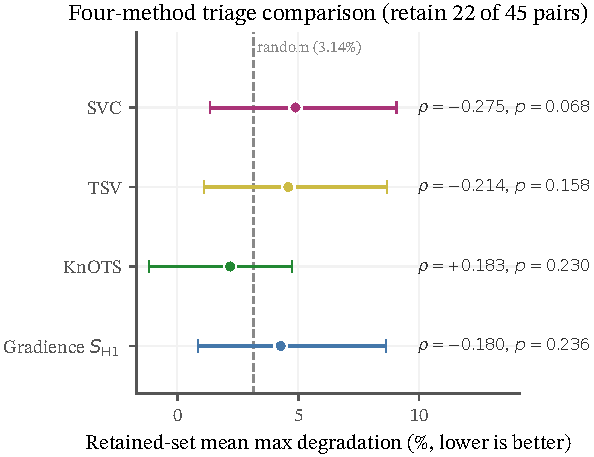
\includegraphics[width=0.8\textwidth]{figures/four_method_forest.pdf}
  \caption{Four-method triage comparison on the 45 evaluated
    cross-task pairs. Methods are ordered by magnitude of Spearman
    $\rho$ between their risk score and max degradation. Horizontal
    error bars are family-pair-blocked bootstrap 95\% CIs on the
    retained-set mean. Vertical dashed line: random-baseline mean
    max degradation (3.14\%) across all 45 pairs. Per-method $\rho$
    and $p$ are annotated inline. No method's CI excludes the random
    baseline. Three of four methods sit visibly to the right of
    baseline (worse than random on retained-set mean degradation);
    KnOTS alone sits to the left with a right-signed $\rho$, but
    its CI crosses baseline.}
  \label{fig:four-method}
\end{figure}

The framework's reading: this is evidence that the measurement
substrate (weight-space spectral geometry) rather than any specific
algorithmic choice within it is the binding constraint on per-pair
prediction at the evaluated scale and sample size. The reading is
honestly flagged as one plausible interpretation rather than a
definitive claim; activation-informed methods (beyond weight-space
alone, e.g., \citep{zhang2025osrm,zhou2026demystifying}) remain an
open direction.

\section{A Previously-Unnamed Measurement Property}
\label{sec:rank-observation}

\subsection{Observation}

Applied to the worked example, the framework prescribes a tiered
reproducibility check across a nontrivial environment gap. On
execution (T6 in the consolidation record), every scalar in the
primary H1 analysis reproduces bit-identical or within float-noise
tolerance ($\leq 10^{-3}$) \emph{except} the headline partial
Spearman $\rho$, which drifts from the committed $-0.533$ to a
reproduced $-0.545$ --- an absolute difference of $1.2 \times
10^{-2}$. The drift is localized: raw Spearman (no residualization)
is bit-identical; $R^2$ of both the family baseline and the full
model is bit-identical; $\Delta R^2$ is bit-identical; bootstrap
quantities drift by at most $2 \times 10^{-3}$. The only non-trivial
drift is in the Spearman statistic applied to OLS residuals.

\subsection{Explanation}

Spearman correlation is a rank-based statistic: it depends on the
pairwise ordering of its inputs, not their magnitudes. At $n = 45$
residuals where many values are close together, a floating-point
perturbation too small to shift the sum of squares by more than its
15th decimal place can still flip the rank order of a few near-tied
residual pairs. Each rank-pair flip shifts Spearman by
$2/(n(n^2-1)) \approx 2.2 \times 10^{-5}$; flipping on the order of
a few hundred near-tied pairs accumulates drift of the observed
magnitude. Across numerical environments, the committed value and
the reproduced value are \emph{both correct}: each is computed
faithfully from the same input data by the same algorithm under
different floating-point paths in \texttt{numpy.linalg.lstsq}.
Neither value is more right than the other. The statistic is
numerically ill-conditioned on residuals of this size at this
sample count.

\subsection{Implication}

The H1 decision is robust to this precision: the partial $\rho$
is approximately $-0.53$ in both environments, decisively below the
$+0.50$ threshold (wrong sign) in both, and the decision (H1 not
confirmed) is identical in both. But the specific point estimate of
partial $\rho$ should be reported as approximately $-0.53 \pm 0.01$
rather than as a four-decimal value. The third decimal is not a real
claim. At $n = 200$ or larger the statistic's intrinsic precision
would stabilize substantially; at $n = 45$, it does not.

\subsection{Generalization}

Rank-based statistics appear widely in ML diagnostic reporting:
Spearman correlations, Kendall's tau, rank-based robustness
metrics, ranked model comparisons. Whenever these are computed on
residuals --- i.e., after controlling for another variable via
regression --- the residualization step is a numerical-precision
amplifier. Any paper reporting such statistics at small sample
sizes without explicitly bounding the precision is making an
implicit claim the data does not support. This is not a one-off
observation about N134; it is a general measurement property the
framework's reproducibility discipline surfaced.

The observation also demonstrates the framework's central claim:
measurement discipline applied to ML diagnostic reporting produces
findings that unstructured reporting does not. The precision
property was not present in the original N134 analysis and was not
present in the committed report; it was surfaced by running the
analysis in a different environment and comparing tier-by-tier
with a tolerance schedule calibrated to quantity class. Without
that discipline, N134 would have reported $-0.533$ to three
decimals indefinitely, and the third decimal would have been an
unstated promise the data could not keep.

\section{Generalizing from the Case Study}
\label{sec:generalizing}

\subsection{Reporting practices the framework prescribes}

Pulled together as a short list suitable for direct adoption:

\begin{enumerate}
  \item Cross-seed ICC or equivalent reliability coefficient
    reported alongside any diagnostic claim intended to support
    quantitative prediction.
  \item Bounded precision with explicit tolerance schedule,
    calibrated per quantity class and per sample size. Rank-based
    statistics on residuals, specifically, should report
    sample-size-calibrated precision bounds.
  \item Confound decomposition with pre-registered decision rules.
    For predictive-correlation claims, the default should be a
    family- or category-residualized partial correlation with a
    $\Delta R^2$ threshold, not a raw correlation.
  \item Floating-point reproducibility check with tiered
    verification (qualitative claims, structural agreement,
    quantitative agreement with tolerance schedule, gap
    documentation). Binary pass/fail is insufficient once the
    reproduction environment is not a controlled copy of
    production.
  \item Post-hoc analyses labeled as such and assigned no
    evidential weight. The C4 pre-registration discipline is
    minimum-viable methodological hygiene.
\end{enumerate}

None of these is mathematically novel; all are mature methods
drawn from classical test theory and its descendants. What the
framework adds is coordination --- applying all five in conjunction
rather than any one in isolation.

\subsection{What this changes about how existing claims should be read}

The framework does not re-adjudicate specific published claims, but
it does argue that readers of the ML methods literature should
calibrate credence to the measurement-discipline practices of
reports rather than to their reported point estimates. A diagnostic
reported as ``Spearman $\rho = 0.572$'' without a cross-seed
distribution, without a family-residualized partial correlation, and
without a reproducibility-check trace is making a weaker evidential
claim than the reported value suggests. Readers should discount
accordingly until the missing measurement-theoretic context is
supplied.

\subsection{Why this is not a critique of any specific paper}

The practices the framework prescribes are not currently normative
in the ML methods literature. Papers not following them are not
violating field norms; they are following the norms that exist.
Our claim is that the norms should change, and that individual
papers should begin applying the framework voluntarily ahead of any
field-wide shift. We apply it ourselves in N134; we do not ask
anyone else to retroactively apply it to work they have already
published.

\subsection{The psychometric-tradition reference}

The framework is drawn directly from classical test theory and its
modern descendants (IRT, generalizability theory, measurement
invariance theory). Canonical references are
\citet{cronbach1951alpha} on reliability,
\citet{shrout1979icc} on ICC,
\citet{messick1989validity,messick1995validity} on construct
validity as unified-theory framework, and
\citet{cronbachmeehl1955} on construct validity and
nomological networks. We are not claiming originality for the
measurement-theoretic concepts; we are claiming that their
systematic application to ML diagnostics is underdeveloped and
proposing a specific framework for that application.

\section{Objections, Alternatives, Limitations}
\label{sec:objections}

\paragraph{``This is just good statistics; nothing psychometric-specific
is needed.''} Classical test theory contains specific machinery
(ICC, SEM, construct validity, convergent and discriminant validity,
generalizability-theory decompositions) that is not covered by
statistics coursework typical in ML training. The framework is
``just good statistics'' in the sense that it is not mathematically
novel; but it is a specific coordinated application of methods that
are not currently coordinated in ML practice. The coordinated
application is the contribution.

\paragraph{``Pre-registration is high-overhead and impractical for
most ML research.''} The N134 experiment ran end-to-end in
approximately 30 hours for \$40 on commercial cloud compute with a
pre-registration written as a single document committed before data
collection. The overhead is lower than typical reviewer-response
cycles in the same literature. The practicality objection reflects
current norms rather than actual cost.

\paragraph{``The worked example is a null; the framework would be
more compelling with a positive result.''} The framework's value is
demonstrated by what it rules out as much as by what it confirms.
A framework that would have licensed a false-positive claim (as the
precursor study's B-P5 analysis almost did
\citep{anonymized2026n133}) is a framework worth adopting. The null
is a feature of the worked example, not a weakness of the framework.
A positive result would demonstrate that the framework survives
non-null outcomes; the present null demonstrates that it survives
the null outcomes where methodological discipline is most tested.

\paragraph{``Rank-on-residuals floating-point sensitivity is a niche
observation; generalizing from it is overreach.''} The observation
is not the paper's center of gravity; it is a demonstration instance
of the framework producing findings unstructured reporting does not.
The generalization is to the class of rank-based statistics on
small-$N$ residuals, which is not niche --- it covers a meaningful
fraction of diagnostic reporting in the ML methods literature
wherever partial rank correlations, rank-based robustness tests, or
ranked comparisons are reported at modest sample sizes.

\paragraph{Limitations proper.} The worked example studies a single
backbone (Mistral-7B-v0.3), a single LoRA rank ($r = 16$), a single
merge operation ($0.5/0.5$ linear), and a single class of diagnostic
metric (weight-space spectral). The framework's claims generalize
beyond these specifics; the worked example's empirical claims do
not. A reader interested in the framework's application to their own
diagnostic class will need to carry out their own application rather
than directly importing N134's results.

\section{Conclusion}
\label{sec:conclusion}

We have argued that ML diagnostic reporting systematically lacks the
measurement-theoretic infrastructure that psychological assessment
has treated as baseline methodology for decades, that this lack
produces overclaims of precision and generality, and that a specific
four-component framework --- construct validity, reliability
coefficients, bounded precision claims with tolerance schedules,
pre-registered confound decomposition --- addresses the gap. The
N134 worked example applies the framework to spectral LoRA-merging
diagnostics at decoder scale under family-confound control,
produces a pre-registered null on per-pair merge prediction,
replicates task-boundary detection across three architectures and
two metric families, and surfaces a previously-unnamed measurement
property (rank-based correlation on small-$N$ residuals has intrinsic
floating-point precision of order $10^{-2}$) that unstructured
reporting would not have produced.

Three directions follow. First, activation-informed analogues of the
worked example's spectral score remain a candidate for exceeding the
regime null the worked example documents (N135-alt). Second, the
framework's specific prescriptions will evolve with application
experience; this paper is a starting point rather than a completed
methodology. Third, individual papers can begin applying the
framework voluntarily ahead of any field-wide shift, and we invite
them to.

% -----------------------------------------------------------------------------
\bibliography{references}

% -----------------------------------------------------------------------------
\appendix

\section{Exact $S_{\mathrm{H1}}$ Score Definition and Decision Rule}
\label{app:score}

For a pair of adapters $(a, b)$ trained on tasks $T_a, T_b$ with
$T_a \neq T_b$, let $U^{(a)}_\ell, \sigma^{(a)}_\ell$ and
$V^{(a)}_\ell$ denote the left singular vectors, singular values, and
right singular vectors of the O-projection of layer $\ell$'s LoRA
update, with analogous quantities for adapter $b$. Define
\begin{equation*}
\alpha^{(O)}_\ell(a, b)
\;=\; \frac{\sum_{i, j} \sigma^{(a)}_i \sigma^{(b)}_j \,
  |\langle u^{(a)}_i, u^{(b)}_j \rangle| \cdot
  |\langle v^{(a)}_i, v^{(b)}_j \rangle|}
{\left(\sum_i (\sigma^{(a)}_i)^2\right)^{1/2}
 \left(\sum_j (\sigma^{(b)}_j)^2\right)^{1/2}}.
\end{equation*}
The primary score is the depth-weighted aggregate,
$S_{\mathrm{H1}}(a, b) = \sum_\ell \ell \cdot \alpha^{(O)}_\ell(a, b) \,/\, \sum_\ell \ell$
over the 32 layers of Mistral-7B-v0.3.

The decision rule requires both criteria:
\begin{enumerate}
  \item Partial Spearman
    $\rho(S_{\mathrm{H1}}^{\perp F}, D^{\perp F}) \geq +0.50$
    at $p < 0.05$, where $\cdot^{\perp F}$ denotes OLS residuals
    after regressing on FAMILY\_B dummies, and $D$ is max
    degradation.
  \item $R^2_{\mathrm{full}} - R^2_{\mathrm{family}} \geq 0.10$,
    where $R^2_{\mathrm{family}}$ is the OLS $R^2$ for
    $D \sim \mathrm{FAMILY\_B}$ and $R^2_{\mathrm{full}}$ is the
    OLS $R^2$ for $D \sim \mathrm{FAMILY\_B} + S_{\mathrm{H1}}$.
\end{enumerate}
Sign constraint is absolute: wrong sign fails regardless of
magnitude.

\section{Bootstrap Protocol}
\label{app:bootstrap}

All confidence intervals are block-bootstrap resampled with blocks
defined by task-family-pair cell (under FAMILY\_B). Each resample
draws with replacement among the 28 family-pair cells and
concatenates all observations within the drawn cells. Reported
intervals use 5,000 resamples; percentile intervals at the 2.5\%
and 97.5\% empirical quantiles.

\section{Pairwise Triage Adaptations of KnOTS, TSV, SVC}
\label{app:adaptations}

The four-method comparison (Section~\ref{sec:empirical}) uses
pairwise-triage adaptations of each method's core measurement
quantity rather than the published reference implementations. We
did not import the published repositories as dependencies; instead,
each of the three score functions in the N134 analysis scripts
computes the quantity that the corresponding paper identifies as its
central interference or inflation signal, aggregated at the pair
level as a triage score. The faithfulness and departure notes are
inline in the score functions' docstrings; full documentation is in
the \texttt{08\_compare\_methods.py} script in the companion
repository. A reviewer who reads ``we used KnOTS'' in
Section~\ref{sec:empirical} should read it as shorthand for ``we
adapted KnOTS's shared-subspace interference-norm quantity to the
pairwise triage setting,'' not as a claim that we executed the
published paper's full pipeline.

\section{Cross-Seed Reliability for $S_{\mathrm{H1}}$}
\label{app:reliability}

Cross-seed ICC(2,1) for $S_{\mathrm{H1}}$, estimated from the 24
same-task adapter pairs (three within-task seed-pairs
$\times$ eight tasks; absolute agreement, single measurement
\citep{shrout1979icc}), is
$\hat{\rho}_{\mathrm{ICC}} = 0.566$, with 95\% CI
$[0.165, 0.874]$ by the Shrout--Fleiss F-distribution method.
A secondary block-bootstrap over tasks (5{,}000 resamples, seed
134) yields CI $[0.141, 0.965]$, which diverges from the
parametric CI by up to 0.091 on the upper bound.
We report both intervals. The divergence is itself informative
about parametric-assumption strain at $N = 8$ tasks and illustrates
that a point estimate with a single CI can understate the
uncertainty about a reliability coefficient at small sample
sizes; this is the kind of limitation the paper argues should be
stated rather than hidden.

The standard error of measurement,
$\mathrm{SEM} = \mathrm{SD}_{\mathrm{pooled}} \sqrt{1 - \hat{\rho}_{\mathrm{ICC}}} = 0.014$,
is the measurement-theoretic precision of a single-seed-pair
same-task $S_{\mathrm{H1}}$ estimate. Against pooled same-task
$S_{\mathrm{H1}}$ values ($\mathrm{SD}_{\mathrm{pooled}} = 0.021$,
range $[0.044, 0.112]$), SEM of $0.014$ is substantial: it states
that the instrument's precision in the regime where the alignment
signal is designed to be large is comparable in magnitude to a
meaningful fraction of the signal itself. Note that the reliability
design targets same-task pairs; transferring the SEM to cross-task-
pair precision claims, which operate in the smaller
$S_{\mathrm{H1}} \in [0.015, 0.025]$ regime, is a broader
inferential step this estimate does not license directly.

$\hat{\rho}_{\mathrm{ICC}} = 0.566$ places the instrument at
``moderate'' cross-seed reliability by the conventional descriptive
thresholds ($>\!0.9$ excellent, $>\!0.75$ good, $>\!0.50$ moderate,
$<\!0.50$ poor). We report the conventional description only as
orientation and not as a binary gate; the paper's framework argues
against thresholding continuous reliability estimates into
verdicts. Full panel, mean-squares decomposition, and bootstrap
details are in
\texttt{sidecar/results/n134/analysis\_icc.json}; design
commitments are documented in
\texttt{sidecar/notes/n134\_icc\_spec.md}.

\section{Full Reproducibility-Check Trace}
\label{app:reproducibility}

Summary of the T6 reproducibility check performed on the committed
N134 state. Full trace in \texttt{n134\_reproducibility\_check.md}
in the companion repository. Protocol: four-tier verification as
specified in Section~\ref{sec:rank-observation} and in the sidecar
convention.

\textbf{Tier 1 (qualitative claims).} All six qualitative claims
reproduce: H1 not confirmed; B-P1, B-P2, B-P4 replications all
confirmed; no N133 composite score exceeds H1 thresholds on N134
data; composite-score sign pattern unchanged across the environment
gap.

\textbf{Tier 2 (structural agreement).} \texttt{analysis\_h1.json}
and \texttt{analysis\_secondary.json} schemas reproduce exactly.

\textbf{Tier 3 (quantitative agreement).} All scalars within the
amended tolerance schedule. One value (partial Spearman $\rho$)
falls into the rank-on-residuals precision regime, drifting by
$1.18 \times 10^{-2}$ between the pod environment ($-0.5330$) and
the dev environment ($-0.5448$). Every other scalar is bit-identical
or at float-precision-noise magnitude. The Phase 5 four-method
comparison cannot be re-verified from committed state alone because
per-adapter SVD factor sidecars were not committed (size constraint;
1.2 GB on pod); the committed \texttt{method\_comparison.json} is
the canonical Phase 5 output.

\textbf{Tier 4 (gap documentation).} Environment gap: Python 3.11
$\rightarrow$ 3.14; \texttt{numpy} 1.26 $\rightarrow$ 2.4;
\texttt{scipy} 1.13 $\rightarrow$ 1.17. Data-availability gap:
Phase 5 per-adapter factor files are pod-only. Both gaps are
documented in the companion reproducibility-check trace; neither
affects qualitative claims.

\section{Deviations from Pre-Registration}
\label{app:deviations}

Six code-level or infrastructure-level deviations were caught before
H1 was computable from committed data. None altered the
pre-registered protocol, task set, training design, $S_{\mathrm{H1}}$
definition, or decision rule. Summary: (D1) transformers API
change; (D2) pair-key ordering mismatch between \texttt{pair\_sample}
and analysis script; (D3) layer-indexing and module-string schema
mismatches; (D4) JSON bool serialization; (D5) CPU-contention
incident during pilot training, with loss-trajectory continuity
verified post-incident; (D6) Phase 5 per-pair v2.1 audit file shape
gap, resolved via a lazy per-pair synthesizer before any
method-comparison numbers were committed. Full deviation records in
the companion repository's \texttt{n134\_incident\_log.md} and
\texttt{n134\_report.md} Section 8.

\section{Compute, Environment, Artifacts}
\label{app:compute}

Single RTX 6000 Ada 48GB on commercial cloud (RunPod Secure Cloud).
End-to-end compute approximately 30 hours at approximately \$40
total cost. Pod software environment: Python 3.11, \texttt{torch}
2.3, \texttt{transformers} 4.44, \texttt{peft} 0.12, \texttt{numpy}
1.26, \texttt{scipy} 1.13 (inferred from commit-time compatibility
fixes; the pod was decommissioned before a \texttt{pip freeze} was
captured; a post-hoc development-environment \texttt{pip freeze} is
provided in the companion repository as a replication starting
point with explicit disclaimer that it is not the pod environment).
All analytical artifacts (pre-registration document, raw audit
JSONs, merge evaluation outputs, analysis scripts, figure-generation
scripts, reproducibility-check trace) are in the companion
repository under tag \texttt{n134-submission-draft-v1}.

\end{document}
